\documentclass[a4paper,11pt]{article}
\usepackage[utf8]{inputenc}
\usepackage[T1]{fontenc}
\usepackage[frenchb]{babel}

\usepackage{graphicx}
\usepackage{fancyhdr}
\usepackage{geometry}

\usepackage[colorlinks,linkcolor=blue]{hyperref}
\usepackage{amsmath}
\usepackage{amssymb}
\usepackage{mathrsfs}
\usepackage{epsfig}
\usepackage {eurosym}

\usepackage{float}

\geometry{a4paper,tmargin=2cm,bmargin=2cm,lmargin=1.5cm,rmargin=1cm,headheight=2.2cm,headsep=0.5cm,footskip=1cm}
\columnsep=0.6cm

\graphicspath{{images/}} 

\usepackage{listings}
\usepackage{color}
\usepackage{xcolor}

\lstset{columns=flexible,keepspaces=true, breaklines,breakindent=0pt} 


\lstset{language=VHDL,
basicstyle=\ttfamily\footnotesize,
breaklines, 
keywordstyle=\bfseries\color{blue},
stringstyle=\color{red},
commentstyle=\color{blue!20!black!30!green},
morecomment=[s][\color{black}]{/**}{*/},
numbers=left,
numberstyle=\tiny\color{black},
stepnumber=2,
numbersep=10pt,
tabsize=4,
showspaces=false,
showstringspaces=false}


\fancypagestyle{plain}{
% noms des respo   dans le bas de page                                            
\lfoot{Projet de VHDL}
\rfoot{M.Morin J.Fourmann}
\renewcommand{\headrulewidth}{0pt}
\fancyhead{}}
% Titre a compl»ter
\title{\textbf{ \huge{Projet de VHDL}}  \\{\Large Réalisation d'un Fréquencemètre}}

\author{
\textsc{Jérémie Fourmann} (Promo 2013 - Eléctronique)\\ %mettre votre nom
\textsc{Maxime Morin} (Promo 2013 - Eléctronique)\\ %mettre votre nom
%\textsc{ddd dddd} (Promo - departement - respo)     %2 nom
}

\graphicspath{{images/}}

\begin{document}

\pagestyle{plain}

\maketitle
\begin{center}

\includegraphics[width=6cm]{inp-enseeiht.pdf}   
\end{center}

\vspace{1cm}
\renewcommand{\contentsname}{Plan}
\tableofcontents
\vspace{2cm}

\newpage
\section{Objectifs}
Le but de ce projet est de meusurer la fréquence d'un signal, le résultat de cette mesure sera affichée sur quatres afficheurs 7 segments.\\
\subsection{Rappel du cahier des charges}
Notre projet doit répondre aux contraintes suivantes :
\begin{description}
 \item[Changement de gamme automatique :] Pour garder le plus de précision possible, 
il faudra changer de méthode de mesure quand la fréquence dépassera une certaine valeur (voir partie nos choix).
\item[Rafraichissement de la mesure de 1s :] Permet de garder une bonne fluidité lorsque la fréquence est ammenée à changer.
\item[Affichage sur 4 digits :] Permet d'avoir une précision correcte
\item[Plage de fréquence de 1Hz à 10 MHz]
\item[Affichage des calibres]  
\end{description}
\vspace{.5cm}
\emph{RQ: Par ailleurs notre système affichera un message d'alerte quand le signal mesuré dépasse la plage de fréquence admise.}

\subsection{Nos choix}
\subsubsection{Choix de la validité des méthodes de mesures}
Nous avons deux méthodes de mesures à notre disposition : méthode étalon et méthode échantillonage.\\
\begin{figure}[H]
\begin{center}
	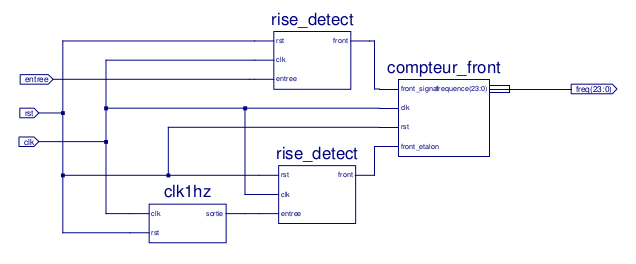
\includegraphics[scale=.3]{etalon.png}
	\caption{Métode étalon}
\end{center}
\end{figure}

\begin{figure}[H]
\begin{center}
	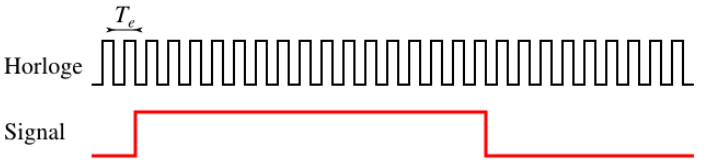
\includegraphics[scale=.3]{ech.png}
	\caption{Méthode échantillonage}
\end{center}
\end{figure}
Ces deux méthodes ne sont pas meilleur l'une que l'autre, elles sont complémentaires.\\
En effet pour un signal de fréquence élevé nous utiliseron la méthode étalon, elle permet d'avoir le maximum de précision.\\
En revanche à basse fréquence cette méthode ne peut s'apliquer convenablement, nous utilisons alors la méthode échantillonage.\\

Il faut donc trouver la valeur pour laquelle on change de méthode de mesure. Nous allons tracer la précision en fonction de la fréquence pour 
les deux méthodes\\
On a :
\begin{equation*}
 Precision_{BF}=\frac{F_{clk}}{F_{signal}}
\end{equation*}
\begin{equation*}
 Precision_{HF}=\frac{F_{signal}}{F_{étalon}}
\end{equation*}

\begin{figure}[H]
\begin{center}
	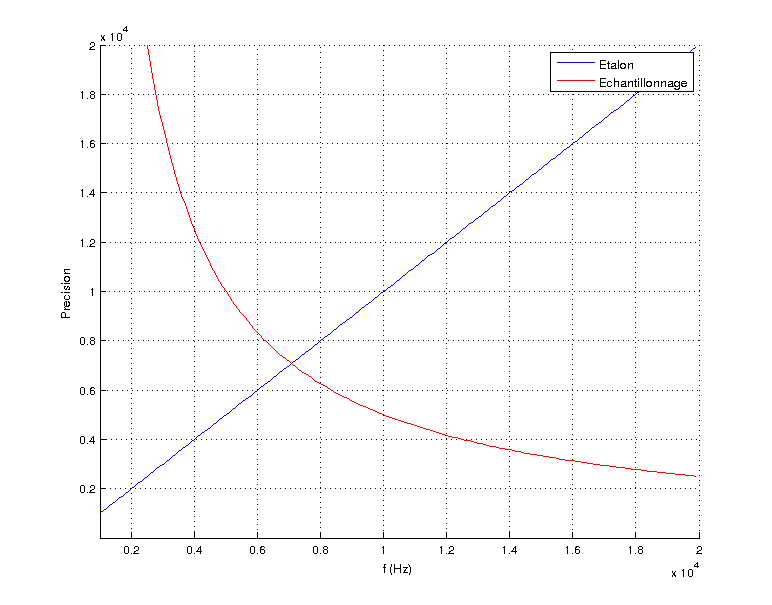
\includegraphics[scale=.5]{graphMethode.png}
	\caption{Précision des deux méthodes}
\end{center}
\end{figure}
On s'aperçoit que pour avoir le maximun de précision il faut changer de méthode aux alentours de 7 KHz. 

\subsubsection{Choix de la conception en machine d'état}
Notre conception étant entièrement synchrone, chaque sous module de notre sytème sera une machine d'état avec le bloc M et G synchronisé sur
la clock du FPGA.\\
Cette conception en machine d'état nous assure une implémentation adapté aux fonctionement du FPGA.\\ 
Par ailleurs nous avons aussi une meilleur lisibilité de notre programme et une meilleur facon de débugger car nous avons accès à l'état de notre machine lors des simulations.\\
\newpage
\section{Conception du système}

\subsection{Présentation du système}

  \paragraph{}Le système final que nous implémenteons sur le FPGA ressemble à ceci :

\begin{figure}[H]
\begin{center}
	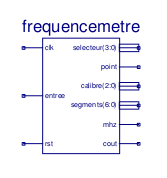
\includegraphics[scale=1]{sch-freqa0.png}
	\caption{Diagramme A-0}
\end{center}
\end{figure}

\paragraph{} L'utilisateur n'aura qu'à envoyer le signal dont il veut mesurer la fréquence. Pour une approche plus technique, décomposons
ce bloc en sours modules :

\begin{figure}[H]
\begin{center}
	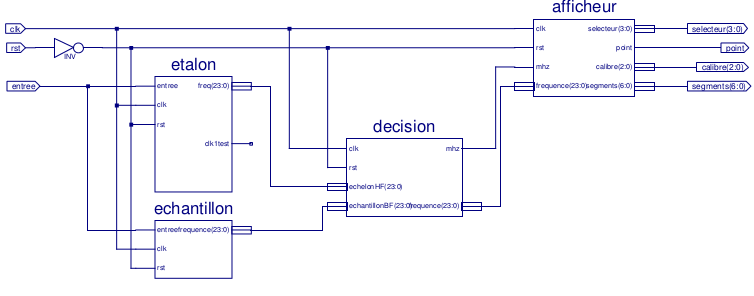
\includegraphics[scale=1]{sch-frequencemetre.png}
	\caption{Diagramme A0}
\end{center}
\end{figure}

\paragraph{} Notre fréquencemètre se décompose en 4 blocs principaux que nous développerons par la suite : 
\begin{description}
  \item[La mesure par étalon : ] Nous mesurons le nombre de fronts du signal pendant une période étalon de 1 seconde. Ce nombre de fronts est
  proportionnel à la fréquence.
  \item[La mesure par échantillonnage] Nous comptons le nombre de fronts d'horloge entre dexus fronts du signal. Ce nombre est
  inversement proportionnel à la fréquence, il faudra l'inverser...
  \item[La décision] Nous choisissons quelle mesure est la plus précise pour être afficher, selon la fréquence de travail...
  \item[L'affichage] Nous affichons la valeur envoyée par le module de décision.
\end{description}

\paragraph{} Par la suite, nous allons détailler ces modules dans le même ordre que nous les avons conçus.

\subsection{Module d'affichage}
  \subsubsection{Schéma bloc}
  
  \begin{figure}[H]
\begin{center}
	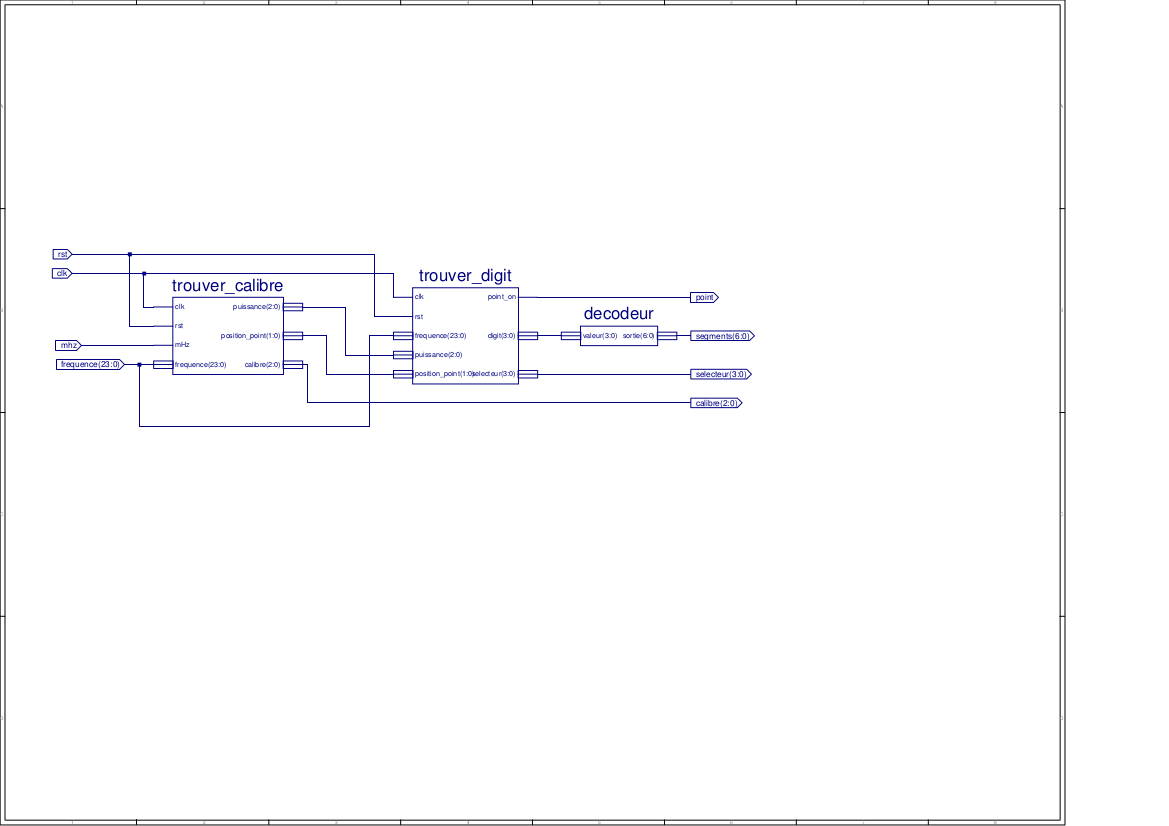
\includegraphics[scale=1]{sch-afficheur.png}
	\caption{Diagramme A1 : module d'affichage}
\end{center}
\end{figure}

\paragraph{} L'objectif de ce module est de transformer le résultat de la mesure (une succession de zéros et de uns sans unités) 
en une grandeur physique en décimale dans les grandeurs du système internationnal... Nous avons choisi de faire un bloc très générique : 
il recevra un nombre binaire codé sur 24 bits et une information sur son unité (Hertz ou milli-Hertz), il devra ensuite le formater 
et l'afficher sur les 4 afficheurs de la carte, en plaçant le point et déterminant le calibre.

\begin{description}
  \item[trouver\_calibre : ] Ce bloc détermine le calibre que nous allons afficher à l'utilisateur, c'est à dire la position du point, la
  led à allumer, et la puissance de 10 du nombre à afficher (utile pour la conversion dans le bloc suivant)
  \item[trouver\_digit : ] Ce module converti en binaire codé décimal et affiche un à un les quatres digits significatifs de la fréquence. 
  Il utilise des données déteminées par le bloc précédent. Il gère aussi le balayage en insérant un reatrd de 2ms entre deux digits et 
  en commandant le sélecteur.
  \item[decodeur : ] Ce bloc se contente de convertir le BCD pour commander l'afficheur.
\end{description}


  \subsubsection{Machines d'états}
  \subsubsection{Résulats de simulation}


\subsection{Mesure par étalon}
  \subsubsection{Schéma bloc}
  
  \begin{figure}[H]
\begin{center}
	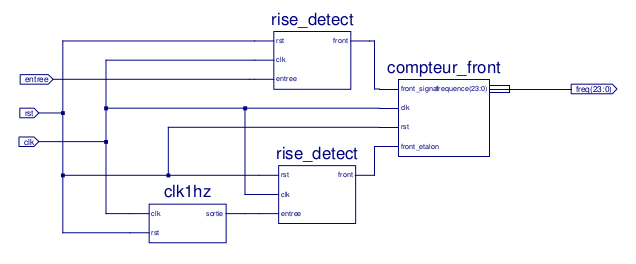
\includegraphics[scale=1]{sch-etalon.png}
	\caption{Diagramme A2 : mesure par étalon}
\end{center}
\end{figure}

\paragraph{} L'objectif de ce module est de compter le nombre de front du signal pendant un temps fixe apellé ``étalon''.
La période de cet étalon a été fixé précédemment (TODO) à une seconde. Etant donné que cette méthode ne sera utilisée que pour les 
fréquences suppérieures au KHz (le seuil étant à 7kHz), nous ferons en sorte que la grandeur de sortie soit en Hz, ce qui nous permet 
de rentrer dans le chaier des chagres en tremes de précison et en terme de plage de fréquence en n'utilisant que 24bits. Ce module 
ferta appel aux sous modules suivants :

\begin{description}
  \item[rise_detect : ] Ce bloc permet de générer une impulsion durant exactement 1 cycle d'horloge lorsqu'un front montant est détecté
  sur son entrée.
  \item[clk1hz : ] Module de division de fréquence permettant de générer une fréquence de 1 Hertz pour cadencer les échelons.
  \item[compteur_fronts : ] Ce bloc compte le nombre de fronts du signal entre deux fronts du signal d'étalon, après chaque mesure,
  il met la valeur sur le bus de sortie et relance une nouvelle mesure.
\end{description}


  \subsubsection{Machines d'états}
  \subsubsection{Résulat de simulation}

  \subsection{Mesure par échantillonnage}
  \subsubsection{Schéma bloc}
  
  \begin{figure}[H]
\begin{center}
	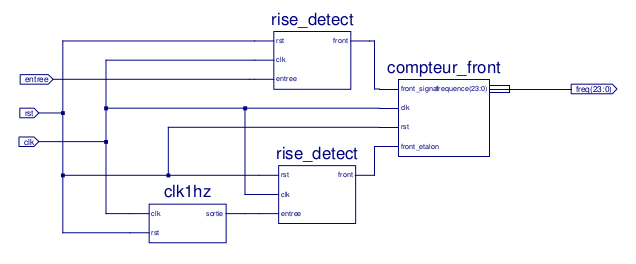
\includegraphics[scale=1]{sch-etalon.png}
	\caption{Diagramme A3 : mesure par étalon}
\end{center}
\end{figure}

\paragraph{} L'objectif de ce module est de compter le nombre de front du signal pendant un temps fixe apellé ``étalon''.
La période de cet étalon a été fixé précédemment (TODO) à une seconde. Etant donné que cette méthode ne sera utilisée que pour les 
fréquences suppérieures au KHz (le seuil étant à 7kHz), nous ferons en sorte que la grandeur de sortie soit en Hz, ce qui nous permet 
de rentrer dans le chaier des chagres en tremes de précison et en terme de plage de fréquence en n'utilisant que 24bits. Ce module 
ferta appel aux sous modules suivants :

\begin{description}
  \item[rise_detect : ] Ce bloc permet de générer une impulsion durant exactement 1 cycle d'horloge lorsqu'un front montant est détecté
  sur son entrée.
  \item[clk1hz : ] Module de division de fréquence permettant de générer une fréquence de 1 Hertz pour cadencer les échelons.
  \item[compteur_fronts : ] Ce bloc compte le nombre de fronts du signal entre deux fronts du signal d'étalon, après chaque mesure,
  il met la valeur sur le bus de sortie et relance une nouvelle mesure.
\end{description}


  \subsubsection{Machines d'états}
  \subsubsection{Résulat de simulation}

\subsection{Performances du système}



\newpage
\section{Bilan}

\newpage
\appendix
\section{Manuel d'utilisateur}
\subsection{Introduction}
L'utilisateur pourra utilisé le projet soit en utilisant le component Fréquencemètre pour l'inclure dans un autre projet soit l'utilisé directement sur la Nexys 2.

\subsection{Component VHDL}
Notre projet peut se résumer en un seul component suivant :


\subsection{Implémentation sur Nexys 2}
En chargent le .bit, l'utilisateur pourra utilisé le fréquencemètre.
\begin{figure}[H]
\begin{center}
	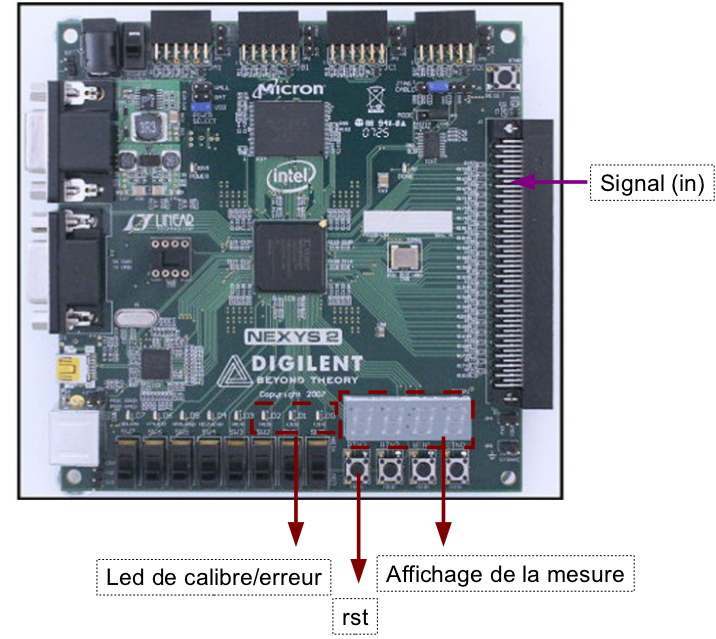
\includegraphics[scale=.5]{fpga.png}
	\caption{Implémentation sur carte Nexys 2}
\end{center}
\end{figure}

\subsection{Fichier contrainte}
L'utilisateur pourra édité le fichier de contraintes selon ses besoins et ressources disponible.
\lstinputlisting{../frequencemetre.ucf}
\newpage
\section{Extrait de code VHDL}
\lstinputlisting{../machine_etat.vhd}
\end{document}
